\documentclass[tikz, margin=2]{standalone}
\usepackage{amsmath}

\begin{document}
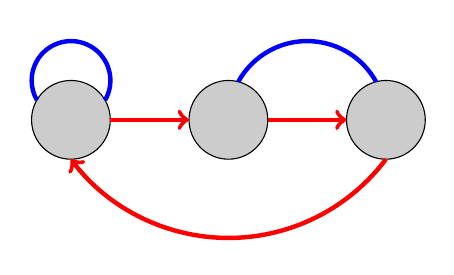
\begin{tikzpicture}

% The three elements of X
\filldraw[fill=gray!40] (-2,0) circle (.5);
\filldraw[fill=gray!40] ( 0,0) circle (.5);
\filldraw[fill=gray!40] ( 2,0) circle (.5);

% Rotations
\draw[red,ultra thick,->] (-1.5,0) -- (-0.5,0);
\draw[red,ultra thick,->] ( 0.5,0) -- ( 1.5,0);
\draw[red,ultra thick,->] (2,-.5) arc (-36.87:-143.13:2.5);

% Flips
\draw[blue,ultra thick] (-1.566,.25) arc (-30:210:.5);
\draw[blue,ultra thick] (1.875,.484) arc (28.955:151.044:1);

\end{tikzpicture}
\end{document}
